
%(BEGIN_QUESTION)
% Copyright 2010, Tony R. Kuphaldt, released under the Creative Commons Attribution License (v 1.0)
% This means you may do almost anything with this work of mine, so long as you give me proper credit

Suppose the low-pressure switch (PSL) in this compressor control system fails shorted (i.e. its contacts can never electrically open):

$$\includegraphics[width=15.5cm]{i02287x01.eps}$$

Explain how this system will act when left in the ``Auto'' mode, given the following pressure switch settings calibrated when the system was first placed into service years ago:

\begin{itemize}
\item{} Cut-out switch = {\it opens at 110 PSI rising, closes at 105 PSI falling}
\vskip 10pt
\item{} PSH = {\it opens at 95 PSI rising, closes at 93 PSI falling}
\vskip 10pt
\item{} PSL = {\it opens at 74 PSI rising, closes at 70 PSI falling}
\end{itemize}

\underbar{file i02287}
%(END_QUESTION)





%(BEGIN_ANSWER)

The receiver tank pressure will cycle between 93 PSI and 95 PSI, with the high-pressure control switch acting as the only control.

%(END_ANSWER)





%(BEGIN_NOTES)

{\bf This question is intended for exams only and not worksheets!}.

%(END_NOTES)

